\chapter{Background Theory}

\section{Introduction to Computer Vision}

\subsection{Introduction}
This chapter contains the background theory which is necessary to understand the implementations in chapter \ref{chp:implementation} and how they are intended to work. 

\subsection{How it's Done}
nanana

\subsection{OpenCV}

OpenCV (Open Source Computer Vision Library) is an  open source library with a vast number of advanced computer vision and machine learning algorithms. The library supports Windows, Linux, iOS and Android, and has interfaces to C, C++, Python, Java and MATLAB. All OpenCV applications in this project uses OpenCV 3.0.0 for Windows. OpenCV for Windows can be downloaded from sourceforge.net. This download contains source files, sample programs, sample data and a pre-built library for MSVC 2010 and 2013. The pre-build library can quickly be plugged into  an IDE such as Qt Creator or Visual Studio 2013, thus giving the programmer access to all basic OpenCV features. A steb-by-step guide for using both the pre-built and a custom-built library can be found in Appendix \ref{}.

\begin{figure}
\centering
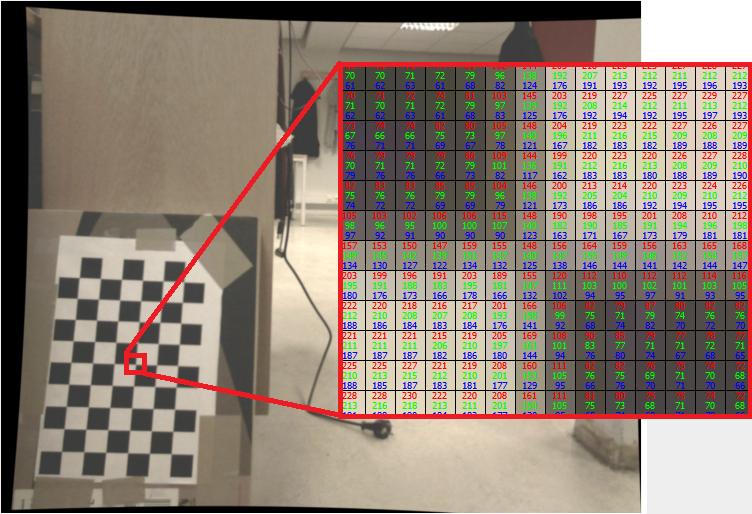
\includegraphics[scale=0.7]{SjakkMat}
\caption{Elements in a cv::Mat representing an image. This is a 3-channel image with 8 bit RGB colors.}
\label{fig:matGrid}
\end{figure}

\section{Stereo Vision and Depth Perception}

Stereo vision and depth perception is one of the core topics within this report. Here, the theory behind a method using two cameras is presented, while some additional methods are mentioned to provide context. 

\subsection{Various Methods}

Methods for depth perception in computer vision can be separated into two main categories, i.e. active and passive. Active sensors will usually project a light pattern onto the scene to be perceived, before sensing how this pattern is displaced by the topology of the scene. The Kinect sensor and 3d-scanners using laser light are typical examples of active sensors. Passive depth perception makes use of many of the same cues we use to perceive depth. The most common passive sensors extract the depth information by observing observing a scene from at least two different positions. 

Optical flow is another important method for depth perception. Optical flow may be either active or passive. The passive variant requires  only one camera, but depends on motion and a stream of images to extract depth information. Observing how much some chosen features in a scene has moved in the image frame at $t = 1$ compared to the frame at $t = 0$ is the basis of depth sensing from optical flow. When the camera moves through a scene where all objects are stationary, objects that are far away will naturally have an optical flow field with a smaller magnitude than objects that are close. 

\subsection{Stereoscopic Vision in General}

In this project, passive stereoscopic vision is achieved by using two identical (in theory) cameras placed on the same plane. The gist of passive stereoscopic vision is based on the fact that objects close to the camera pair will have a large displacement from the left to the right camera compared to objects that are further away. This concept is illustrated in figure \ref{fig:3dScene}.

\begin{figure}
\centering
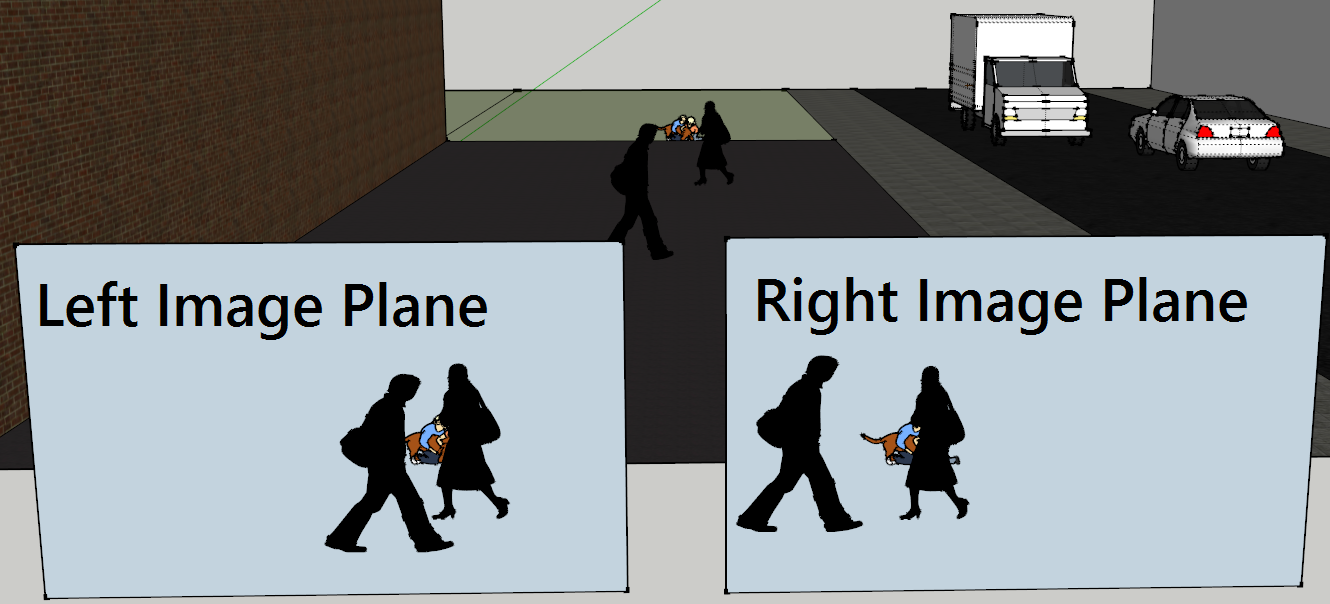
\includegraphics[scale=0.4]{3dScene}
\caption{\label{fig:3dScene}Left to right displacement on the image plane based on distance.}
\end{figure} 

\paragraph{The Pinhole Camera Model}

Figure \ref{fig:pinhole} illustrates the geometry of a pinhole camera. In a pinhole camera, a scene will be projected onto an image plane, often denoted $\pi$, through the camera projection point $O$ which is located at the origin. The focal length $f$ is the distance from the projection point $O$ to the image plane $\pi$. In a true pinhole camera the image plane will be located behind the lens and the projection point $O$, and the scene projection will be rotated by $180^{\circ}$. A virtual image plane placed in front of $O$ is intended to make the figure more straightforward. 

\begin{wrapfigure}{r}{0.6\textwidth}
    \vspace{-10pt} % Remove exessive whitespace
    \centering
    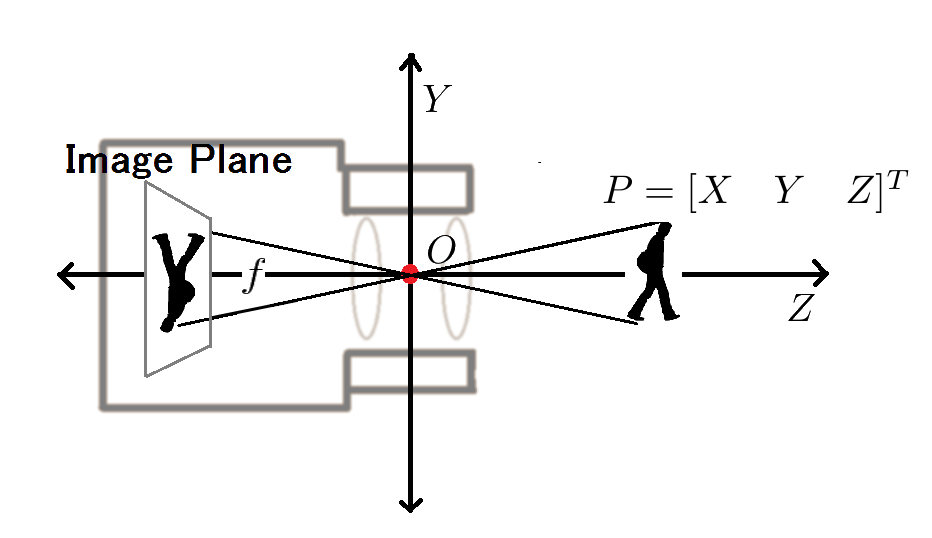
\includegraphics[width=0.6\textwidth]{pinhole}
    \caption{Geometry of a pinhole camera.}
    \vspace{-10pt} % Remove exessive whitespace
    \label{phantompic}
\end{wrapfigure}

\paragraph{Stereo Cameras}

Figure \ref{fig:StereoSpace} shows an ideal stereo camera model.  The model comprise two pinhole camera models where the virtual image planes are located on the same plane. The two image planes are separated by a horizontal translation $B$ which is called the baseline. This implies that the projection point $O_L$  in the left camera, relates to the projection point $O_R$ on the right camera through $B$: $O_R = O_L + B$. Each of the two image planes has a left handed pixel based coordinate system $u,v$, i.e. the origin is in the top left corner and the opposite pixel is in the bottom right corner. 

\begin{figure}
\centering
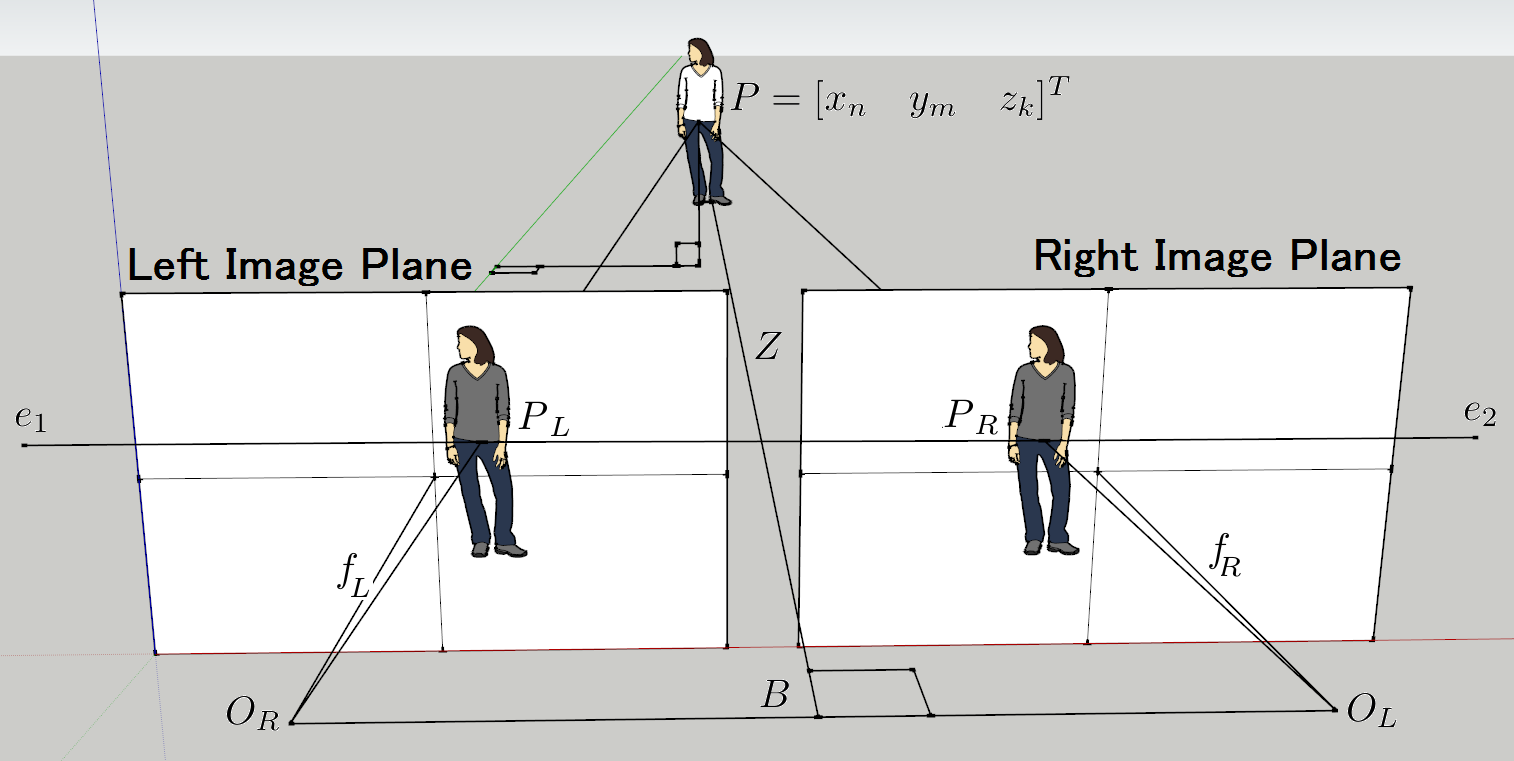
\includegraphics[width=1\textwidth]{StereoSpace}
\caption{\label{fig:StereoSpace}Geometry of stereo vision.}
\end{figure}

\paragraph{Camera Distortion}

Cite \cite{einstein}.

\subsection{Stereoscopic Vision in OpenCV}

The prebuilt version of OpenCV 3.0.0 comes with two stereo matching algorithms: Block Matching (StereoBM) and Semi Global Block Matching (StereoSGBM). Additional algorithms are available if OpenCV is built with, e.g. CUDA.

\paragraph{StereoSGBM}\cite{hirschmullerstereo}
blablabalb
